\documentclass[12pt,a4paper]{scrartcl}
\usepackage[utf8]{inputenc}
\usepackage[english,russian]{babel}
\usepackage{misccorr}
\usepackage{graphicx}
\usepackage{amsmath}
\usepackage{amsfonts}
\usepackage{verbatim}
\usepackage{listings}
\usepackage{pgfplots}
\usepackage{graphicx}
\usepackage{pdfpages}
\usepackage{multirow}

\DeclareUnicodeCharacter{03BC}{\ensuremath{\mu}}
\DeclareUnicodeCharacter{03B3}{\ensuremath{\gamma}}
\DeclareUnicodeCharacter{03C3}{\ensuremath{\sigma}}
\DeclareUnicodeCharacter{03B8}{\ensuremath{\theta}}
\DeclareUnicodeCharacter{03C7}{\ensuremath{\chi}}
\DeclareUnicodeCharacter{03B1}{\ensuremath{\alpha}}

\usepackage{algorithm}
\usepackage{algpseudocode}

% Настройки листингов.
% 8 Листинги

\usepackage{listings}

% Значения по умолчанию
\lstset{
  language=[Sharp]C,
  basicstyle= \footnotesize,
  breakatwhitespace=true,% разрыв строк только на whitespacce
  breaklines=true,       % переносить длинные строки
%   captionpos=b,          % подписи снизу -- вроде не надо
  inputencoding=koi8-r,
  numbers=left,          % нумерация слева
  numberstyle=\footnotesize,
  showspaces=false,      % показывать пробелы подчеркиваниями -- идиотизм 70-х годов
  showstringspaces=false,
  showtabs=false,        % и табы тоже
  stepnumber=1,
  tabsize=4,              % кому нужны табы по 8 символов?
  frame=single,
  commentstyle=\color{green},
  morekeywords={partial, var, value, get, set},
  keywordstyle=\color{blue},
  stringstyle=\color{red}
}

% Стиль для псевдокода: строчки обычно короткие, поэтому размер шрифта побольше
\lstdefinestyle{pseudocode}{
  basicstyle=\small,
  keywordstyle=\color{black}\bfseries\underbar,
  language=Pseudocode,
  numberstyle=\footnotesize,
  commentstyle=\footnotesize\it
}

% Стиль для обычного кода: маленький шрифт
\lstdefinestyle{realcode}{
  basicstyle=\scriptsize,
  numberstyle=\footnotesize
}

% Стиль для коротких кусков обычного кода: средний шрифт
\lstdefinestyle{simplecode}{
  basicstyle=\footnotesize,
  numberstyle=\footnotesize
}

% Стиль для BNF
\lstdefinestyle{grammar}{
  basicstyle=\footnotesize,
  numberstyle=\footnotesize,
  stringstyle=\bfseries\ttfamily,
  language=BNF
}

% Определим свой язык для написания псевдокодов на основе Python
\lstdefinelanguage[]{Pseudocode}[]{Python}{
  morekeywords={each,empty,wait,do},% ключевые слова добавлять сюда
  morecomment=[s]{\{}{\}},% комменты {а-ля Pascal} смотрятся нагляднее
  literate=% а сюда добавлять операторы, которые хотите отображать как мат. символы
    {->}{\ensuremath{$\rightarrow$}~}2%
    {<-}{\ensuremath{$\leftarrow$}~}2%
    {:=}{\ensuremath{$\leftarrow$}~}2%
    {<--}{\ensuremath{$\Longleftarrow$}~}2%
}[keywords,comments]

% Свой язык для задания грамматик в BNF
\lstdefinelanguage[]{BNF}[]{}{
  morekeywords={},
  morecomment=[s]{@}{@},
  morestring=[b]",%
  literate=%
    {->}{\ensuremath{$\rightarrow$}~}2%
    {*}{\ensuremath{$^*$}~}2%
    {+}{\ensuremath{$^+$}~}2%
    {|}{\ensuremath{$|$}~}2%
}[keywords,comments,strings]

% Подписи к листингам на русском языке.
\renewcommand\lstlistingname{Листинг}
\renewcommand\lstlistlistingname{Листинги}


\begin{document}
\begin{titlepage}
\newpage
\begin{center}
Федеральное государственное бюджетное образовательное учреждение  \\
\vspace{0.25cm}%расстояние до верхней строчки
высшего образования «Московский государственный технический  \\
\vspace{0.25cm}%расстояние до верхней строчки
университет имени Н.Э.Баумана (национальный исследовательский \\
\vspace{0.25cm}%расстояние до верхней строчки
университет)» (МГТУ им. Н.Э.Баумана) \\
%\hrulefill %горизонтальная черта
\end{center}
\vspace{5cm}
\begin{center}
\Large Отчёт по лабораторной работе №2 \\ По дисциплине «Математическая статистика» \\ Тема: «Интервальные оценки» \\ Вариант: 1
\end{center}
%\vspace{2.5em}
\vspace{6em}
\begin{flushright}
Студент: \hrulefill Барсуков Н.М. \\
\vspace{1.5em}
Группа: \hrulefill ИУ7-62\\
\vspace{1.5em}
Преподаватель: \hrulefill Саркисян П.С.\\
\vspace{1.5em}
\end{flushright}
\vspace{\fill}
\begin{center}
Москва, 2020
\end{center}
\end{titlepage}
\newpage
\tableofcontents
\addcontentsline{toc}{section}{Введение}
\newpage
\begin{center}
\textbf {Введение}
\end{center}

Цель работы: построение доверительных интервалов для математического ожидания и дисперсии нормальной случайной величины.

Содержание работы:
\begin{enumerate}
	\item для выборки объёма n из нормальной генеральной совокупности X реализовать в виде программы на ЭВМ:
	\begin{enumerate}
		\item вычисление точечных оценок $\hat{μ}(\overrightarrow {x_n})$ и $S^2(\overrightarrow {x_n})$ математического ожидания $MX$ и дисперсии $DX$ соответственно;
		\item вычисление нижней и верхней границ $\underline {μ}(\overrightarrow {x_n})$, $\overline {μ}(\overrightarrow {x_n})$ для γ-доверительного интервала для математического ожидания $MX$;
		\item вычисление нижней и верхней границ $\underline {σ}^2 (\overrightarrow {x_n})$, $\overline {σ}^2 (\overrightarrow {x_n})$ для γ-доверительного интервала для дисперсии $DX$;
	\end{enumerate}
	\item вычислить $\hat{μ}$ и $S^2$ для выборки из индивидуального варианта;
	\item для заданного пользователем уровня доверия γ и N - объёма выборки из индивидуального варианта:
	\begin{enumerate}
		\item на координатной плоскости $O_{yn}$ построить прямую $y = \hat{μ}(\overrightarrow {x_N})$, также графики функций $y = \hat{μ}(\overrightarrow {x_n})$, $y = \underline {μ}(\overrightarrow {x_n})$ и $y = \overline {μ}(\overrightarrow {x_n})$ как функций объёма n выборки, где n изменяется от 1 до N;
		\item на другой координатной плоскости $O_{zn}$ построить прямую $z = S^2(\overrightarrow {x_N})$, также графики функций $z = S^2(\overrightarrow {x_n})$, $z = \underline {σ}^2 (\overrightarrow {x_n})$ и $z = \overline {σ}^2 (\overrightarrow {x_n})$ как функций объёма n выборки, где n изменяетя от 1 до N.
	\end{enumerate}
\end{enumerate}

\newpage
\addcontentsline{toc}{section}{Теоретическая часть}
\begin{center}
\textbf {Теоретическая часть}
\end{center}

Пусть $\overrightarrow {X_n}$ - случайная выборка объёма n из генеральной совокупности X с функцией распределения $F(X; θ)$, которая зависит от параметра θ, значение которого неизвестно.

Предположим, что для параметра θ построен интервал $(\underline {θ}(\overrightarrow {X_n}); \overline {θ}(\overrightarrow {X_n}))$, где $\underline {θ}(\overrightarrow {X_n})$ и $\overline {θ}(\overrightarrow {X_n})$ являются функциями случайной выборки $\overrightarrow {X_n}$, такой, что выполняется равенство $P\{\underline {θ}(\overrightarrow {X_n}) < θ < \overline {θ}(\overrightarrow {X_n}) \} = γ$.

Интервал $(\underline {θ}(\overrightarrow {X_n}); \overline {θ}(\overrightarrow {X_n}))$ называют интервальной оценкой для параметра θ с коэффициентом доверия γ, а $\underline {θ}(\overrightarrow {X_n})$ и $\overline {θ}(\overrightarrow {X_n})$ называют, соответственно, нижней и верхней границами интервальной оценки. Интервальная оценка $(\underline {θ}(\overrightarrow {X_n}); \overline {θ}(\overrightarrow {X_n}))$ представляет собой интервал со случайными границами, который с заданной вероятностью γ накрывает неизвестное истинное значение параметра θ.

\underline {Определение}: γ-доверительным интервалом (доверительным интервалом с коэффициентом вероятности γ) называют пару статистик  $\underline {θ}(\overrightarrow {X_n})$, $\overline {θ}(\overrightarrow {X_n})$ таких, что для оцениваемого параметра θ $P\{\underline {θ}(\overrightarrow {X_n}) < θ < \overline {θ}(\overrightarrow {X_n}) \} \ge γ$.

Формулы для вычисления границ γ-доверительного интервала для математического ожидания и дисперсии нормальной случайной величины представлены в таблице:

\begin{table}[ht]
	\caption{Формулы для вычисления границ γ-доверительного интервала для математического ожидания и дисперсии нормальной случайной величины}
	\begin{tabular}{|l|c|c|}
		\hline
		Параметры & Центральная статистика & Границы\\
		\hline
		\multirow{2}{*}{μ - неизв., σ - изв.; оценить μ} & \multirow{2}{*}{$\frac {μ - \overline {X}} {σ} * \sqrt{n} \sim N(0,1)$} & $\underline {μ} (\overrightarrow {X_n}) = \overline {X} + \frac {h_α * σ} {\sqrt {n}}$\\
		& & $\overline{μ} (\overrightarrow {X_n}) = \overline {X} + \frac {h_{1-α} * σ} {\sqrt {n}}$\\
		\hline
		\multirow{2}{*}{μ, σ - неизвестны; оценить μ} & \multirow{2}{*}{$\frac {μ - \overline {X}} {S^2(\overrightarrow {x_N})} * \sqrt{n} \sim St(n - 1)$} & $\underline {μ} (\overrightarrow {X_n}) = \overline {X} - \frac {{h^t}_{1-α} * σ} {\sqrt {n}}$\\
		& & $\overline{μ} (\overrightarrow {X_n}) = \overline {X} + \frac {{h^t}_{1-α} * σ} {\sqrt {n}}$\\
		\hline
		\multirow{2}{*}{μ, σ - неизвестны; оценить $σ^2$} & \multirow{2}{*}{$\frac {S^2(\overrightarrow {x_N})} {σ^2} * (n - 1) \sim χ^2(n - 1)$} & $\underline {σ^2} (\overrightarrow {X_n}) = \frac {S^2(\overrightarrow {X_n}) * (n - 1)} {h^{χ^2(n - 1)}_{1-α}}$\\ 
		& & $\overline {σ^2} (\overrightarrow {X_n}) = \frac {S^2(\overrightarrow {X_n}) * (n - 1)} {h^{χ^2(n - 1)}_α}$\\
		\hline
	\end{tabular}
	\label{tab:tabular}
\end{table}

$γ = 1 - 2 * α$, $h_α$ - квантиль уровня α нормального распределения, ${h^t}_α$ - квантиль уровня α распределения Стьюдента, $h^{χ^2(n - 1)}_α$ - квантиль уровня α распределения $χ^2$.

\underline {Определение}: статистика $g(\overrightarrow{X}, θ)$ называется центральной, если закон её распределения не зависит от закона распределения θ, то есть функция распределения $F_g(X)$ не зависит от θ.

Пусть $\overrightarrow {X_n}$ - случайная выборка объёма n из генеральной совокупности X, распределённой по нормальному закону с параметрами μ и ${σ^2}$. Тогда оценить математическое ожидание при неизвестной дисперсии можно следующим образом:

\begin{equation}\label{eq1.1}
\underline {μ} (\overrightarrow {X_n}) = \overline {X} - \frac {S(\overrightarrow {X_n}) * t_{1-α} (n - 1)} {\sqrt {n}};
\end{equation}

\begin{equation}\label{eq1.2}
\overline {μ} (\overrightarrow {X_n}) = \overline {X} + \frac {S(\overrightarrow {X_n}) * t_{1-α} (n - 1)} {\sqrt {n}},
\end{equation}

где $\overline {X}$ - оценка математического ожидания, n - число опытов, $S(\overrightarrow {X_n})$ - точечная оценка дисперсии, $t_{1-α} (n - 1)$ - квантиль уровня (1 - α) для распределения Стьюдента с (n - 1) степенями свободы, $α = \frac {1 - γ} {2}$.

Дисперсию в данном случае можно оценить следующим образом:

\begin{equation}\label{eq1.3}
\underline {σ^2} (\overrightarrow {X_n}) = \frac {S^2(\overrightarrow {X_n}) * (n - 1)} {χ^2_{1-α}(n - 1)};
\end{equation}

\begin{equation}\label{eq1.4}
\overline {σ^2} (\overrightarrow {X_n}) = \frac {S^2(\overrightarrow {X_n}) * (n - 1)} {χ^2_α(n - 1)},
\end{equation}

где n - объём выборки, $χ^2_α(n - 1)$ - квантиль уровня α для распределения $χ^2$ с (n - 1) степенями свободы, $α = \frac {1 - γ} {2}$.

\newpage
\addcontentsline{toc}{section}{Листинг программы}
\begin{center}
\textbf {Листинг программы}
\end{center}

Текст программы $(labwork2.m)$:

\begin{verbatim}
function lab2()
X = [-0.23,-1.03,-4.11,-0.65,-2.58,-0.79,-1.53,
-0.18,-2.79,-1.97,-2.21,-1.59,-0.22,-3.18,-1.18,
-1.42,-1.29,-2.22,-0.82,-1.87,-2.30,-0.94,-0.74,
-2.45,-1.40,-2.09,-0.68,0.02,-1.80,-2.25,-1.19,
-2.17,-1.89,-1.14,-1.50,-1.76,-0.69,-2.21,-1.65,
-1.51,-2.11,-2.24,-0.72,0.94,-0.67,-2.44,-2.27,
-1.33,-3.03,-0.42,-2.86,-2.00,-1.37,-1.90,-2.80,-0.89,
-2.04,-1.66,-0.14,-2.79,-0.21,-1.29,-2.81,-0.29,-1.55,
-0.45,-1.16,-3.96,-3.77,-3.36,-1.81,0.13,-2.61,-3.69,
-3.00,-2.61,-0.74,-0.41,-0.78,-1.49,-1.89,-1.24,-0.00,
-2.72,-1.69,-1.25,-1.59,0.20,-1.08,-2.42,-3.14,-2.54,
-2.09,-2.51,-2.65,-2.42,-1.30,-0.65,1.40,-2.33,-1.97,
-0.54,-1.13,-2.04,0.77,-1.03,-1.55,-1.47,-0.09,-2.11,
-2.08,-1.79,-1.36,-1.92,-3.04,-1.08,-1.67,-2.11,-1.99,-1.64]


N = 1:length(X);

gamma = 0.9;
alpha = (1 - gamma)/2;

mu = expectation(X);
sSqr = variance(X); 

fprintf('mu = %.4f\n', mu); 
fprintf('S^2 = %.4f\n\n', sSqr);

muArray = expectationArray(X, N);
varArray = varianceArray(X, N);

figure
plot([N(1), N(end)], [mu, mu], 'm');
hold on;
plot(N, muArray, 'g');

Ml = muArray - sqrt(varArray./N).*tinv(1 - alpha, N - 1);
plot(N, Ml, 'b');

fprintf('mu_low = %.4f\n', Ml(end));

Mh = muArray + sqrt(varArray./N).*tinv(1 - alpha, N - 1);
plot(N, Mh, 'r'), legend('y=mu', 'y=mu_n', 'y=mu-low_n', 'y=mu-high_n');
grid on;
hold off;

fprintf('mu_high = %.4f\n', Mh(end));

figure
plot([N(1), N(end)], [sSqr, sSqr], 'm');
hold on;
plot(N, varArray, 'g');

Sl = varArray.*(N - 1)./chi2inv(1 - alpha, N - 1);
plot(N, Sl, 'b');

Sh = varArray.*(N - 1)./chi2inv(alpha, N - 1);
plot(N, Sh, 'r'), legend('z=S^2', 'z=S^2_n', 'z=S^2-low_n', 'z=S^2-high_n');
grid on;
hold off;


fprintf('sigma^2_low = %.4f\n', Sl(end));
fprintf('sigma^2_high = %.4f\n', Sh(end));
end

function mu = expectation(X)
mu = mean(X);
end

function sSqr = variance(X)
sSqr = var(X);
end

function muArray = expectationArray(X, N)
muArray = zeros(1, length(N));
for i = 1:length(N)
muArray(i) = expectation(X(1:N(i)));
end
end

function varArray = varianceArray(X, N)
varArray = zeros(1, length(N));
for i = 1:length(N)
varArray(i) = variance(X(1:N(i)));
end
end
\end{verbatim}

\newpage
\addcontentsline{toc}{section}{Результаты расчётов для выборки из индивидуального варианта}
\begin{center}
\textbf {Результаты расчётов для выборки из индивидуального варианта}
\end{center}

Для выборки объёма 120 и $γ = 0.9$ согласно варианту были получены:

\begin{enumerate}
	\item точечные оценки математического ожидания $\hat{μ}(\overrightarrow {x_n})$ и дисперсии $S^2(\overrightarrow {x_n})$;
	\item нижняя и верхняя границы γ-доверительного интервала для математического ожидания $(\underline {μ}(\overrightarrow {x_n}); \overline {μ}(\overrightarrow {x_n})) = (-1.7585; -1.4507)$;
	\item нижняя и верхняя границы γ-доверительного интервала для дисперсии $(\underline {σ}^2 (\overrightarrow {x_n}); \overline {σ}^2 (\overrightarrow {x_n})) = (0.8460; 1.2979)$;
	\item выборочное среднее $ \hat{μ} = -1.6046$;
	\item несмещённая выборочная дисперсия  $S^2 = 1.0341$.
\end{enumerate}

В результате проведённых вычислений для выборки объёма 120 и $γ = 0.9$ согласно варианту были построены соответствующие графики. На графике \ref{graph2.1} представлены прямая $y = \hat{μ}(\overrightarrow {x_N})$ (голубая линия), полученное значение математического ожидания $y = \hat{μ}(\overrightarrow {x_n})$ (красная линия), нижняя граница доверительного интервала $y = \underline {μ}(\overrightarrow {x_n})$ (жёлтая линия) и верхняя граница доверительного интервала $y = \overline {μ}(\overrightarrow {x_n})$ (фиолетовая линия), на графике \ref{graph2.2} - прямая $z = S^2(\overrightarrow {x_N})$ (голубая линия), полученное значение несмещённой дисперсии $z = S^2(\overrightarrow {x_n})$ (красная линия), нижняя интервальная граница $z = \underline {σ}^2 (\overrightarrow {x_n})$ (жёлтая линия) и верхняя интервальная граница $z = \overline {σ}^2 (\overrightarrow {x_n})$ (фиолетовая линия).
\begin{figure}[H]
	\centering
	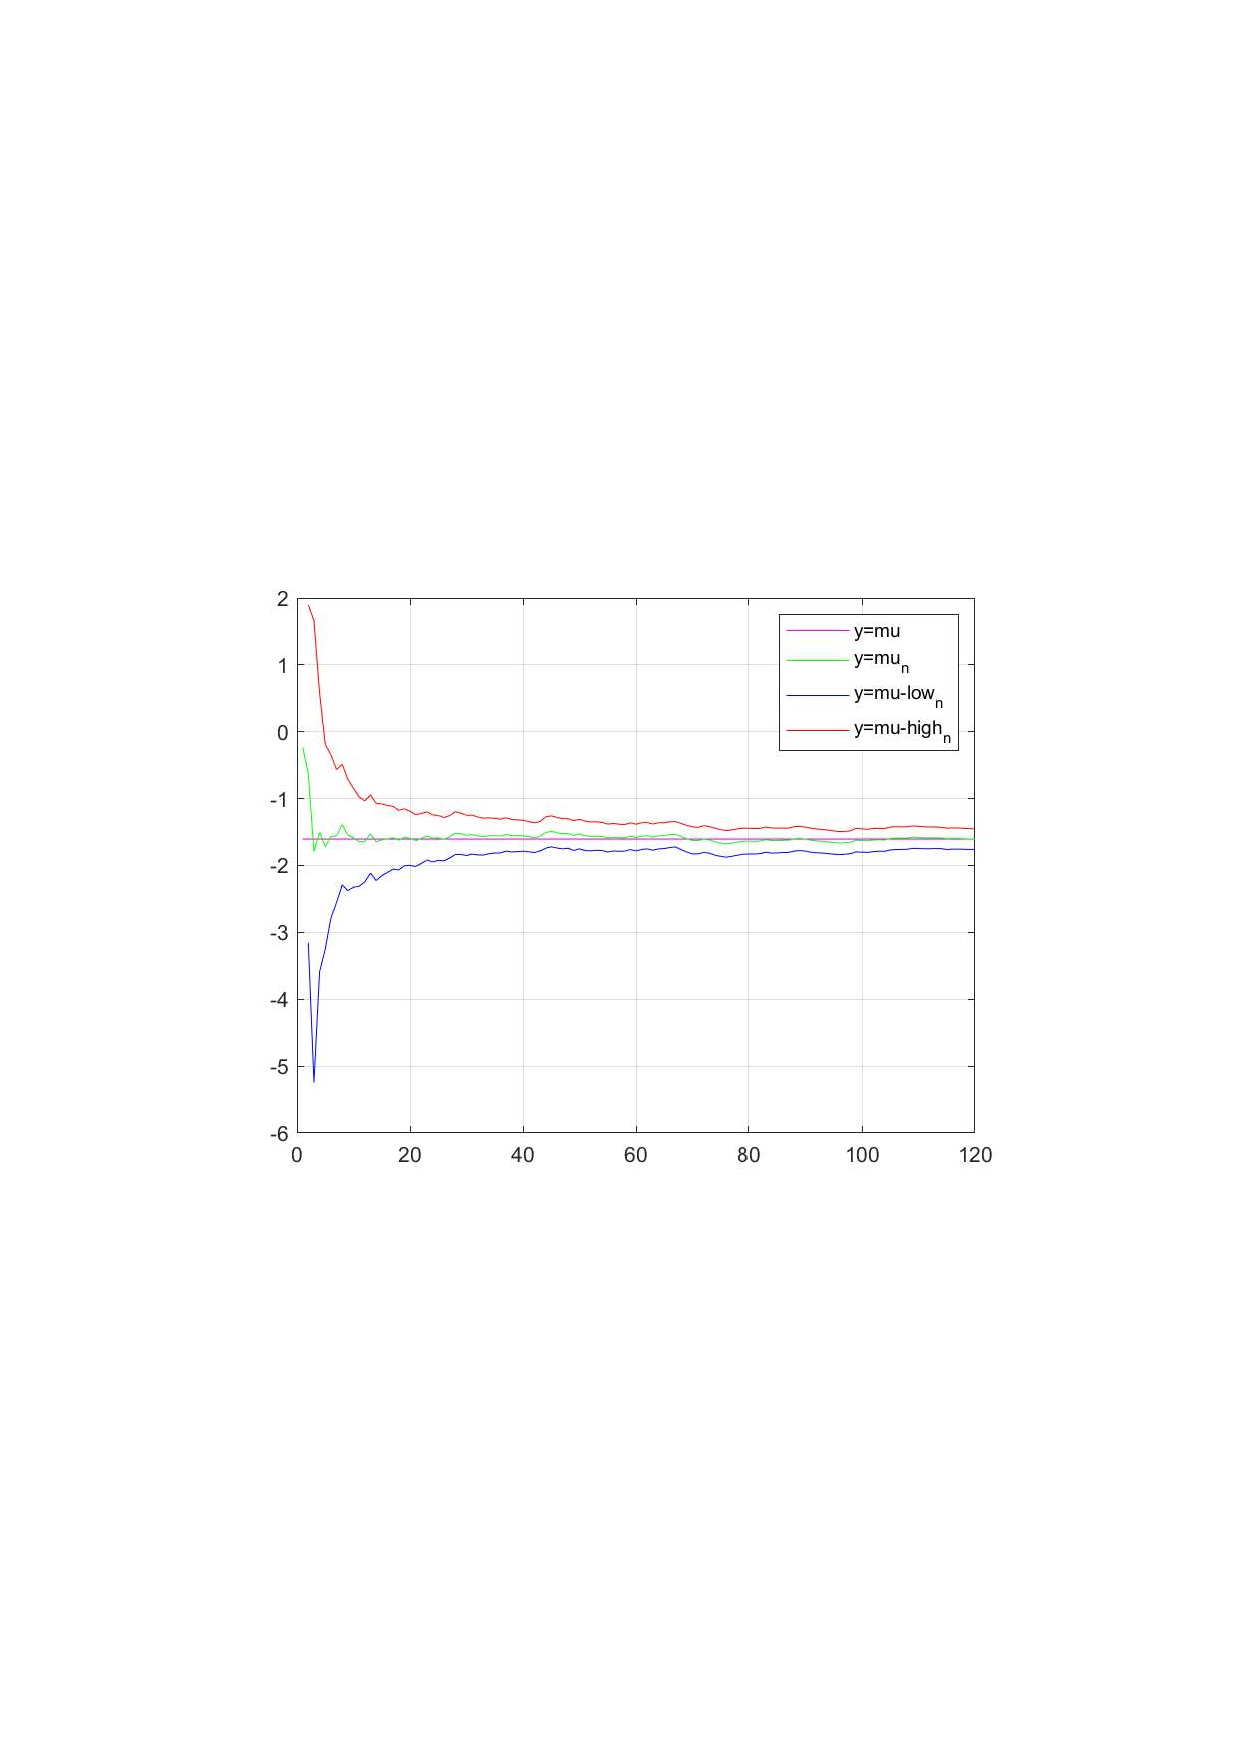
\includegraphics[width=335px]{2.pdf}
	\caption{График доверительного интервала для математического ожидания}
	\label{graph2.1}
\end{figure}

\begin{figure}[H]
	\centering
	
\includegraphics[width=335px]{1.pdf}
	\caption{График доверительного интервала для дисперсии}
	\label{graph2.2}
\end{figure}

\newpage
\addcontentsline{toc}{section}{Заключение}
\begin{center}
\textbf {Заключение}
\end{center}
В результате выполнения лабораторной работы для заданной согласно варианту выборки были получены точечные оценки математического ожидания и дисперсии, границы γ-доверительных интервалов математического ожидания и дисперсии, выборочное среднее, несмещённая выборочная дисперсия. Для выполнения вычислений был написан код MatLab, позволяющий вычислить искомые величины и построить графики γ-доверительных интервалов.

\end{document}